\section{Protein States}

The dynamic behavior of membrane proteins, particularly their ability to adopt multiple conformational states, provides a crucial mechanism for implementing ECC's principles. These protein states represent more than simple on-off switches; they create a rich repertoire of possible configurations that can encode and process information while maintaining direct connection to physical energetics \cite{Balchin2016}. The sophisticated transitions between these states enable neural systems to achieve both stability and flexibility in conscious processing.

Ion channels demonstrate remarkable complexity in their conformational dynamics, maintaining multiple conductance states that respond to various cellular signals \cite{Henzler-Wildman2007}. Rather than operating as simple gates, these proteins transition through numerous functional configurations influenced by voltage, ligand binding, and mechanical forces. This diversity of possible states enables sophisticated regulation of neural activity while providing mechanisms for maintaining stable patterns of network function. The precise control of these conformational changes proves essential for supporting conscious processing.

Receptor proteins exhibit even greater sophistication in their state transitions, integrating multiple inputs through complex patterns of allosteric regulation \cite{Nussinov2013}. Individual receptors can adopt numerous configurations that shape both their binding properties and downstream signaling effects. These varied states enable cells to perform complex computations at the molecular level while maintaining energetic efficiency. The resulting molecular computation occurs through physical state changes rather than abstract symbol manipulation.

Structural proteins contribute to conscious processing through their own complex state dynamics \cite{Frauenfelder2009}. Rather than serving as static scaffolds, these proteins undergo continuous conformational changes that respond to and influence cellular activity. Their dynamic assembly states and force-sensitive configurations enable sophisticated regulation of cellular architecture while supporting stable neural function. This molecular flexibility proves crucial for maintaining the physical organization necessary for conscious processing.

The energetic aspects of protein states take on particular significance within ECC's framework \cite{Karplus2005}. Each conformational state represents a distinct energy minimum within a complex landscape of possible configurations. Transitions between states follow specific energetic pathways that enable reliable information processing while maintaining thermodynamic efficiency. The precise organization of these energy landscapes through evolution has created molecular systems capable of supporting conscious processing.

The coupling between protein states and cellular energy dynamics creates sophisticated systems for information processing grounded in physical transitions \cite{Zhou2008}. Rather than operating through abstract representations, neural computations emerge from actual changes in molecular configuration that remain directly connected to energy flows. This physical basis for information processing proves essential for understanding how conscious systems maintain coherent states while enabling dynamic responses to changing conditions.

\begin{figure}[h]
    \centering
    
\includegraphics[width=0.8\textwidth]{images/protein.png}

    \caption{Depiction of a long strand of a protein.}
\end{figure}

Receptor oligomers reveal particularly complex patterns of state transitions in their molecular organization \cite{Lindorff-Larsen2016}. These protein assemblies can adopt various configurations depending on their molecular environment and activation state, creating rich possibilities for information encoding through physical states. The cooperative interactions between subunits enable sophisticated integration of multiple signals while maintaining stable functional properties. Their precise molecular architecture allows for both sensitivity to specific inputs and resistance to random fluctuations.

The stoichiometry of protein complexes plays a crucial role in determining their possible state transitions \cite{Brangwynne2015}. The precise ratios of different protein subunits within receptor complexes and ion channels shape both their functional properties and energy requirements. These molecular relationships establish specific constraints on how proteins can transition between states while maintaining stable function. The resulting balance between flexibility and stability proves essential for supporting conscious processing.

Post-translational modifications add another layer of control to protein state dynamics \cite{Wright2015}. Chemical modifications like phosphorylation can rapidly alter protein conformations, creating additional possibilities for information encoding through molecular states. These modifications enable cells to adjust protein function in response to ongoing activity while maintaining overall stability. The sophisticated regulation of protein states through chemical modification provides mechanisms for both rapid signaling and sustained changes in cellular properties.

The relationship between protein states and local electric fields demonstrates remarkable sophistication in neural information processing \cite{Tokuriki2009}. Membrane proteins respond to changes in electrical potential through precise conformational changes that alter their functional properties. These voltage-dependent state transitions enable rapid signaling while maintaining energetic efficiency. The resulting coupling between electrical activity and protein conformation creates fundamental mechanisms for neural computation through physical state changes.

The integration of protein states across multiple scales reveals fundamental principles about how biological systems achieve conscious processing \cite{Thirumalai2017}. From individual molecules to cellular assemblies, sophisticated state transitions enable complex information processing while maintaining direct connection to physical energy dynamics. This understanding suggests that consciousness emerges not from abstract computation but from precisely organized patterns of molecular state changes that support both stability and adaptability.

The crowded cellular environment introduces additional complexity to protein state dynamics \cite{Roh2017}. Molecular crowding effects influence both the stability of different conformational states and the kinetics of transitions between them. This physical constraint shapes how proteins function within the dense cellular milieu while providing additional mechanisms for regulating their behavior.

\begin{figure}[h]
    \centering
    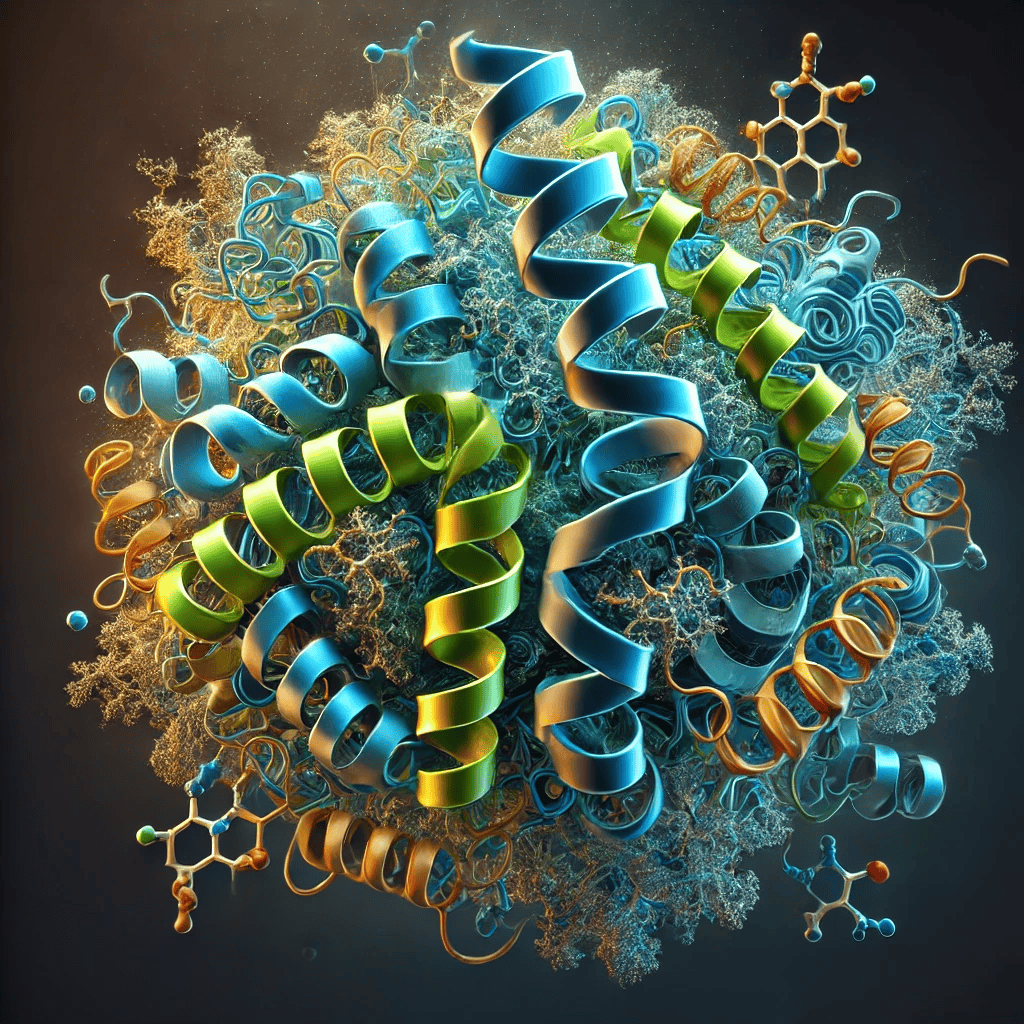
\includegraphics[width=0.8\textwidth]{proteins.png}

    \caption{Proteins can take on exotic conformations}
\end{figure}

Perhaps most significantly, the study of protein states through ECC's framework reveals how information processing can remain grounded in physical transitions while achieving remarkable computational sophistication \cite{Oldfield2014}. Rather than requiring abstraction into symbolic representation, neural computation occurs through actual changes in molecular configuration that maintain direct connection to energy flows. This perspective challenges purely computational approaches to consciousness while suggesting new directions for developing artificial systems capable of supporting conscious-like processing.

The implications extend beyond neuroscience to fundamental questions about the nature of information processing in biological systems \cite{Davis2018}. The remarkable sophistication of protein state dynamics demonstrates how evolution has refined molecular mechanisms to support both stable conscious states and flexible adaptation to changing conditions. This deeper appreciation of molecular complexity proves essential for any complete theory of consciousness and suggests new approaches to treating disorders of conscious processing.

The relationship between protein states and neural energetics reveals fundamental principles about biological computation \cite{Erickson2009}. The precise organization of conformational landscapes enables sophisticated information processing while maintaining direct connection to physical energy flows. This grounding in molecular dynamics helps explain how conscious systems achieve both stability and flexibility through carefully orchestrated patterns of state transitions \cite{Royer2006}.

Moving beyond individual proteins to examine direct cellular coupling, we must now consider how gap junctions enable coherent state maintenance across neural tissues. These specialized channels, composed of connexin proteins, create electrical synapses that allow for rapid, bidirectional communication between cells, proving essential for maintaining the coherent energy states necessary for conscious processing.